\documentclass[%
 reprint,
 amsmath,amssymb
 aps,
]{revtex4}

\usepackage{float}

\usepackage{subfig}
\usepackage{graphicx}% Include figure files
\usepackage{dcolumn}% Align table columns on decimal point
\usepackage{bm}% bold math
\usepackage{physics}
\setlength{}{}%
\usepackage{siunitx}
\usepackage[inline]{asymptote}
\usepackage{multirow}
\usepackage{tikz}
\usepackage{pgfplots, pgfplotstable}
\usepackage{hyperref}
\usepackage{natbib}
\usepackage{amsthm}
\usepackage{amssymb}
\usepackage{amsmath}
\usepackage{cancel}
\bibliographystyle{unsrtnat}
\pgfplotsset{compat=1.3}

\usepackage{pdfpages}

\theoremstyle{remark}
\newtheorem*{rem}{Remark}
\newtheorem*{note}{Note}
\newtheorem{claim}{Claim}

\begin{document}
\title{PHY372: Numerical Simulations of All Photonics Quantum Repeaters}
\author{QiLin Xue}
\maketitle
\tableofcontents
\vspace{4mm}
\section{TODO}
What needs to be done for rough draft 
\begin{itemize}
    \item All the relevant graphs:
    \begin{itemize}
        \item [DONE] $P_cn$ graph 
        \item rate envelope graph
        \item rate vs distance graph
    \end{itemize}
    \item Optimal parameter table
    \item Talk about what measurements need to be done
\end{itemize}
\newpage
\section{Introduction}
Modern cryptography make the fundamental assumption involving the hardness of certain mathematical problems. Challenges related to factoring large numbers or resolving discrete logarithms serve as the basis for security in traditional cryptography - a foundation which, admittedly, has functioned well for many years. However, with the advent of quantum computing and the potential for exponentially increased computational power, many of these classical systems could be cracked. While research into post-quantum cryptography is being made, their security cannot be proven.
\vspace{2mm}

Quantum cryptography works on principles that are fundamentally different from their classical counterparts. One key aspect where they differ is that quantum cryptography uses the features of quantum systems, specifically superposition, and the fact that these states cannot be cloned, protecting them against potential eavesdroppers. Techniques such as the decoy state protocol are unique to quantum cryptography and promise to unlock a higher level of safeguarding information. A basic method within this field is the use of the BB84 protocol with Einstein-Podolsky-Rosen (EPR) pairs, which offers fundamentally secure encryption, as any attempt to intercept communication disturbs the system and reveals the eavesdropper.
\vspace{2mm}

The strength of quantum cryptographic systems also rests on their ability to distribute EPR pairs across large distances - a capability that becomes a technical challenge due to channel loss and noise that increases with distance. This problem, for classical signals, is typically resolved using classical repeaters that amplify the signals to overcome loss and degradation in the transmission medium. Yet, this approach fails when applied to quantum signals due to the 'no cloning theorem' that prevents the replication of quantum states, making the traditional signal-boosting methodology impossible for quantum information transmission.
\begin{figure}[H]
    \centering
    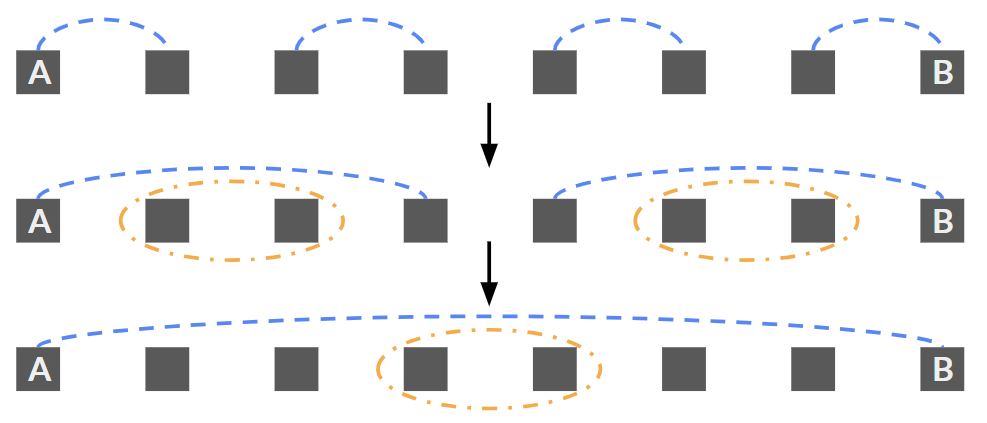
\includegraphics[width=0.7\linewidth]{figs/quantum-repeater.png}
    \caption{A schematic of the quantum repeater with $8$ repeater stations. The dashed blue lines show entangled pairs. When a bell state measurement (BSM) are done, shown in orange, entanglement swapping occurs.}
    \label{fig:QR}
\end{figure}

This is where quantum repeaters come into play. Quantum repeaters, unlike their classical counterparts, do not amplify the quantum signal, but instead, creates long-distance entanglement linking distant nodes through a process known as entanglement swapping, as shown in figure \ref{fig:QR}.
\subsection{Motivation}
The standard repeater protocol is impractical for two major reasons. First, it requires a quantum memory, as each repeater node needs to wait for nearby nodes to be finished before performing the bell state measurements. Second, it requires the ability to convert between stationary qubits (where one can apply quantum operations) and flying qubits (where one can send from one physical location to another).
\vspace{2mm}

While there are suggestions for how to create a quantum memory, such as in the DLCZ protocol, the second problem is very hard. In fact, it is listed as part of DiVencenzo's two extra conditions for a quantum computer. Therefore, building a successful quantum repeater may be just as hard as building a quantum computer. 
\vspace{2mm}

Luckily, there are methods to get around this by modifying the repeater architecture using photonics to avoid the problems associated with quantum memory. Similar techniques are also employed in photonics-based quantum computing.
\section{All-Photonics Quantum Repeater}
\subsection{Brief Overview}
The all photonics quantum repeater makes several improvements from the basic quantum repeater. First, it makes use of several channels for creating entanglement. Since creating these EPR pairs is probabilistic, using several channels ensures a higher chance of success. Failure only occurs if the photon gets lost in all the channels. Error correction techniques, which are discussed in detail later, are able to still guarantee successful entanglement even if only one of the channels at each repeater station successfully receive a photon.
\begin{figure}[h!]
    \centering
    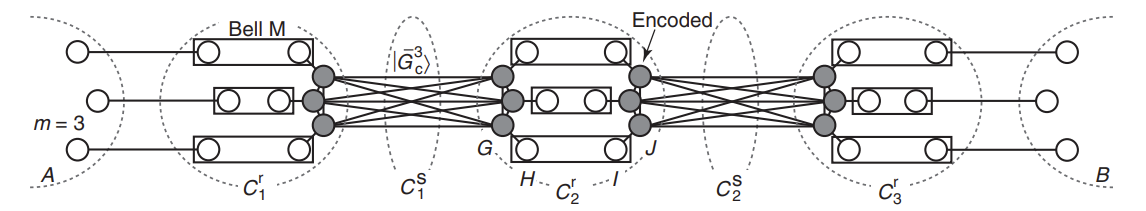
\includegraphics[width=0.8\linewidth]{figs/photonics.png}
    \caption{CAPTION THIS}
    \label{fig:photonics}
\end{figure}
Most importantly though, the method of creating entangled pairs do not require memory at all. Borrowing inspiration from the time-reversed EPR protocol (which ultimately leads to material-device-independent (MDI) QKD). In between each of the $n$ repeater nodes (receiver nodes) lie source nodes, as shown in figure \ref{fig:photonics}. All of Alice, Bob, and the $n-1$ source nodes prepares EPR pairs and sends a photon from each pair to the nearest receiver nodes. For Alice and Bob, they only send one photon from each pair and keep the other. The photons that they keep will eventually be maximally entangled with each other. 

\subsection{Constructing a Graph}
A photonic cluster state is a graph $G(V,E)$ that is prepared by initializing each vertex with a photon prepared in the $\ket{+}$ state and preparing the controlled edge operation of 
\begin{equation}
    \ket{0}\bra{0} \otimes I + \ket{1}\bra{1}\otimes \sigma_Z
\end{equation}
% For example, a fully connect clique of two nodes will become 
% \begin{align}
%     & \frac{1}{\sqrt{2}} \cdot \left(\ket{00} + \ket{01} + \ket{10} +\ket {11}\right) \\ 
%     \mapsto & \frac{1}{\sqrt{2}} \cdot \left(\ket{00} +\ket{01} + \ket{10} - \ket{11}\right)
% \end{align}
For example, a fully connected clique of three nodes will become 
\begin{align}
    & \frac{1}{\sqrt{8}} \cdot \left(\ket{000}+\ket{001}+\ket{010}+\ket{011}+\ket{100}+\ket{101}+\ket{110}+\ket{111}\right) \\ 
\mapsto & \left(\ket{000}+\ket{001}+\ket{010}-\ket{011}+\ket{100}+\ket{101}+\ket{110}-\ket{111}\right) & \text{qubit 2-3}\\ 
\mapsto & \left(\ket{000}+\ket{001}+\ket{010}-\ket{011}+\ket{100}-\ket{101}+\ket{110}+\ket{111}\right) & \text{qubit 1-3} \\
\mapsto & \left(\ket{000}+\ket{001}+\ket{010}-\ket{011}+\ket{100}-\ket{101}-\ket{110}-\ket{111}\right) & \text{qubit 1-2}
\end{align}
where the most significant bit is marked as qubit 1. The advantage of this process is that the state is invariant under the operator
\begin{equation}
    X_i \prod_{j\in \mathcal{N}(i)}Z_j, 
\end{equation}
where $\mathcal{N}(i)$ is the set of neighbours of qubit $i.$ In the 3-qubit example, we can WLOG take $i=1$ and compute,
\begin{align}
    & \left(\ket{000}+\ket{001}+\ket{010}-\ket{011}+\ket{100}-\ket{101}-\ket{110}-\ket{111}\right) \\ 
    \mapsto & \left(\ket{000}-\ket{001}-\ket{010}-\ket{011}+\ket{100}+\ket{101}+\ket{110}-\ket{111}\right) \\ 
    \mapsto & \left(\ket{100}-\ket{101}-\ket{110}-\ket{111}+\ket{000}+\ket{001}+\ket{010}-\ket{011}\right),
\end{align} 
where we can verify is equal to the original state by simple term matching. This invariance property allows \textit{indirect} measurement. If any node $n \in \mathcal{N}(i)$ was lost, we can still infer the result of $Z_n$ by performing the operation $X_i \prod_{j\in \mathcal{N}(i), j\neq n} Z_j.$ This gives a lot of potential for error correction by creating several correlations between qubits.
% https://sci-hub.se/https://journals.aps.org/prl/abstract/10.1103/PhysRevLett.97.120501
\subsection{Photonic Tree}
One major challenge of an all photonics quantum repeater is to construct these trees. Specifically, to protect against loss via error correction, we wish to construct figure \ref{fig:cluster}
\begin{figure}[h!]
    \centering
    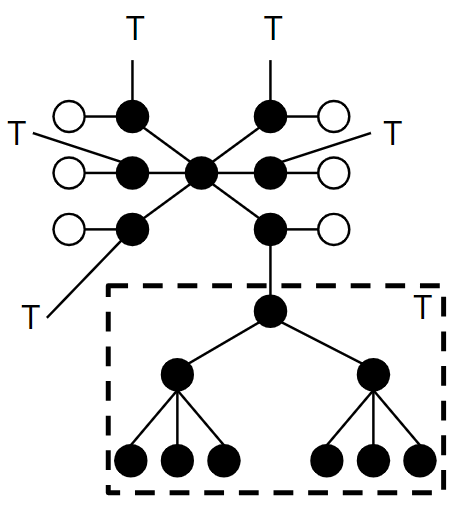
\includegraphics[width=0.25\linewidth]{figs/cluster.png}
    \caption{The quantum tree that needs to be constructed at each repeater node. It consists of a central node in the middle connected to $2m$ nodes. Each of these nodes are connected to a tree $T$ and an outer node (which is the qubit that is transmitted between stations). The tree depicted in this figure has a branching vector of $\vec{b}=[2,3]$ and a depth of $d=2.$}
    \label{fig:cluster}
\end{figure}
where the attached tree has a branching vector of $\vec{b}=[b_0, b_1, \dots, b_d].$ Here, $d$ is the depth of the tree. Later on, we will see that the optimal depth is $d=2,$ as depicted in figure \ref{fig:cluster}. 

This report will discuss and analyze two different ways of constructing such a graph. One using a naive method and one using an improved version.
\subsection{Building a Cluster State}
\textcolor{red}{[\textbf{TODO: example of how to do it}]}
The general idea is to create the needed GHZ states, and combine them to create intermediate states. The states are combined using Fusion II gates \textcolor{red}{\textbf{[INSERT CITATION]}} which removes two photons in the process. That is, combining two states of $x$ photons will result in a state with $2x-2$ photons. That is, if $N(\ell)$ is the number of photons in each cluster tree at the feed-forward stage $\ell,$ then it satisfies the recursive relationship
\begin{equation}
    N(\ell) = 2N(\ell - 1) - 2.
\end{equation} 
Using the initial condition of $N(0)=3,$ we obtain the maximum possible number of photons in the final stage, after $k$ feed-forward steps, as
\begin{equation}
    N(k) = 2^k + 2.
\end{equation}
Note that this is the maximum number because additional measurements can be done in the $Z$-basis which will destroy photons. If a $\vec{b}=[b_0,b_1]$ tree is attached to the central cluster, then the total number of photons is given by 
\begin{equation}
    2m(b_0b_1+b_0+1)+(1+4m)
\end{equation} 
where $b_0b_1+b_0+1$ is the number of photons on each tree and $1+4m$ is the number of photons in the central cluster. This gives us a restriction relating $b_0,b_1,m,k$ together,
\begin{equation}
    2^k + 2 \ge 2m(b_0b_1+b_0+1)+(1+4m).
    \label{eq:kmb-relation}
\end{equation}
\subsection{Basic Mechanisms}
The fundamental building block of creating these cluster states is with Greenberger-Horne-Zeilinger (GHZ) states, given by the maximally entangled state,
\begin{equation}
    \ket{\psi} = \frac{1}{\sqrt{2}}\left(\ket{000}+\ket{111}\right).
\end{equation} 
This is represented by the graph $G(V=3,E=2)$ \textcolor{red}{\textbf{TODO: FIX INCONSISTENCY HERE}}. The probability of successfully generating a GHZ state is
\begin{equation}
    P_\text{GHZ} = \frac{1}{32}\left[\eta_s\eta_d(2-\eta_s\eta_d)^3\right]^3
\end{equation}
where $\eta_s\eta_d$ characterizes the efficiency of the source detector, and should be close to unity. The transmittance of these GHZ states are is given by 
\begin{equation}
    \eta_\text{GHZ} = \frac{\eta_s\eta_d}{2-\eta_s\eta_d}.
\end{equation}
The probability that the photons survive on the chip in a given clock cycle is given by
\begin{equation}
    P_\text{chip} = e^{-\beta\tau_sc_\text{ch}}
\end{equation}
where $c_\text{ch}$ is the speed of light on the chip, $\tau_s$ is the feed-forward time on the chip, and $\beta$ is the on-chip loss coefficient. These parameters can be picked such that the probability the phootn survives in the fiber in one clock cycle, $P_\text{chip} = e^{-\alpha \tau_f c_f}$, is the same. Here, $\alpha$ is another loss coefficient and $\tau_f,c_f$ are the feed-forward time and speed of light in the fiber, respectively.
\textbf{TODO}
\begin{itemize}
    \item Talk about \textbf{clock cycle}
\end{itemize}
\section{Naive Approach}
Let us define 
\begin{itemize}
    \item $P_\text{GHZ}$ is the success probability of creating a $GHZ$ state.
    \item \textcolor{red}{[\textbf{TODO: finish}]}
\end{itemize}
\subsection{Probability Computation}
The general idea is to create the needed GHZ states, and combine them to create intermediate states. The states are combined using Fusion II gates \textcolor{red}{\textbf{[INSERT CITATION]}} which removes two photons in the process. That is, combining two states of $m$ photons will result in a state with $2m-2$ photons.
\vspace{2mm}

However, because creating GHZ states and performing fusion operations are probabilistic, we may need to attempt these operations with multiple copies at each stage. That is, if $n_\text{GHZ}$ GHZ states are attempted, the probability that at least one of them is successful is given by
$$P_0 = 1 - (1 - P_\text{GHZ})^{n_\text{GHZ}}$$
where $1-P_\text{GHZ}$ is the probability of a failure, so $(1 - P_\text{GHZ})^{n_\text{GHZ}}$ is the probability that everything fails. The probability of fusion being successful is given by 
\begin{equation}
    Q_\ell = \frac{1}{2} \cdot (\eta_\text{GHZ}P^{\ell}_\text{chip})^2
\end{equation}
where $\frac{1}{2}$ is the probability under ideal circumstances, and $P_\text{chip}^{\ell}$ is the probability a photon survives on the chip through $\ell$ feed-forward steps. Because we need two photons at this stage, this is squared. The probability of creating the cluster $C^{\ell}_i$ is given by the recursive formula 
\begin{equation}
    P_\ell = 1 - (1 - P^2_{\ell - 1} Q_{\ell})^{n_B},
\end{equation}
where $n_B$ is the number of attempts to create that cluster. For each attempt, the success probability is given by $P^2_{\ell - 1} Q_{\ell}$ because we need both previous cluster states to be available, and the fusion needs to be successful.
\vspace{2mm}

In the final stage, a total of $4m+1$ measurements are made, and the probability of those measurements succeeding is given by
\begin{equation}
    P' = (\eta_\text{GHZ}P_{chip}^{k+1})^{4m+1}
\end{equation} 
since each photon needs to survive $\ell = k+1$ feed-forward cycles. Because these measurements are done on several copies (specifically $n_\text{meas}$ copies), the probability that at least one of them succeeds is given by
\begin{equation}
    P_{c1} = 1 - (1-P_kP')^{n_\text{meas}}.
\end{equation}
Note that in the original paper, the probability was written as $P_\text{c1} = 1 - (Q_kP')^{n_\text{meas}}.$ This is a typo. Because there are $n$ repeater stations, the total probability of all of them succeeding is given by 
\begin{equation}
    P_\text{cn} = P_{c1}^n.
\end{equation}
\subsection{Optimization}
A total of $6n_\text{GHZ}$ photons are needed to create the GHZ states. In each of the $k$ stages, we need $2$ ancillary photons for each of the $n_B$ attempts. A total of $n_\text{meas}$ $C^k$ clusters are attempted, so the total number of photon sources needed at each repeater node is given by
$$ N_s = 6n_\text{GHZ}n_\text{meas} \cdot (2n_B)^k$$
photons. \textcolor{red}{[\textbf{TODO: this isn't the most clear lol}]}
\begin{figure}[h!]
    \centering
    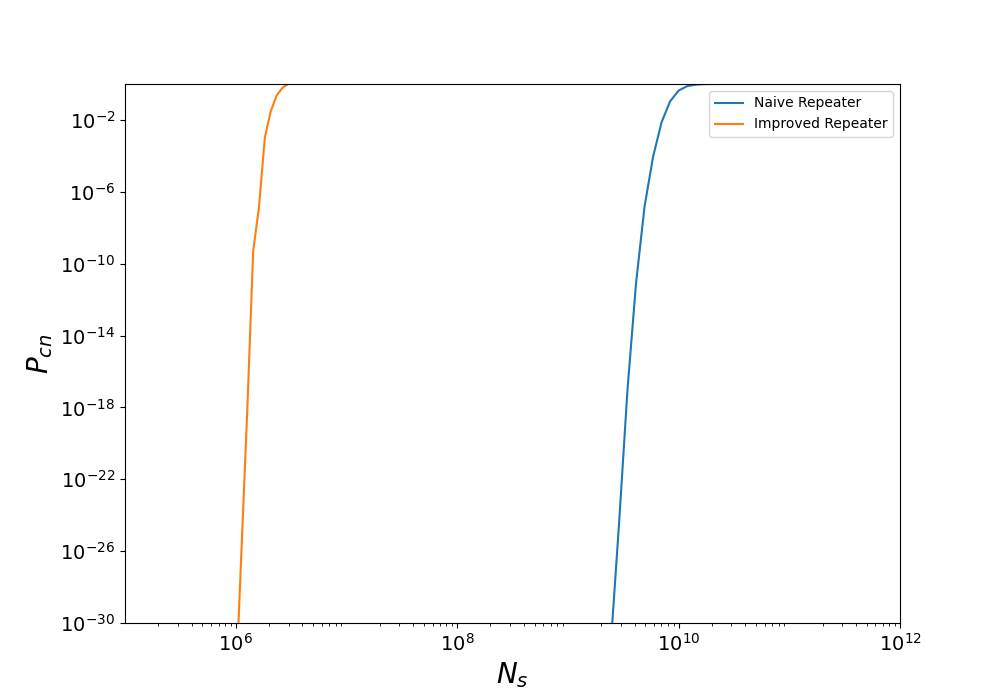
\includegraphics[width=0.6\linewidth]{figs/p_graph.png} 
    \caption{CAPTION THIS}
    \label{fig:p_graph}
\end{figure}
Given a specific $N_s,$ we can find the optimal probability $P_\text{cn}$ by optimizing the three user parameters: $n_B,n_\text{meas},n_\text{GHZ}.$ The probability computations are straightforward to do, so this can be done via a grid search. The result of the optimization is shown in figure \ref{fig:p_graph}.
\section{Improved Approach}
The major drawback of the naive approach is that there is a lot of wasted clusters. For example, if there were three successful intermediate clusters created, only one would go towards the next step. The other two would be wasted, even if it might be needed somewhere else. The improved approach addresses this problem by creating a bank of intermediate cluster states, and fusion steps can choose between any of them.
\vspace{2mm}

Additionally, another major improvement was to move the $4m+1$ basis measurements to be much earlier on, as switching the order of basis measurements and fusion II operations do not matter.\textcolor{red}{[\textbf{TODO: Ned citation for this}]}
\vspace{2mm}

If we start off with $N_s$ photons, then we're attempting to create $\lfloor N_s/6\rfloor$ GHZ states, each with a probability of $P_\text{GHZ}.$ Since these probabilities are identical and independent, the distribution of GHZ states follow a binomial distribution,
\begin{equation}
    B(x, \lfloor N_s/6\rfloor, P_\text{GHZ})
\end{equation}
These GHZ states are distributed into $2^k$ banks $C^0_{i_1,\dots,i_k}.$ These banks are then paired up, and fusion II operations are done to create the $2^{k-1}$ possible different $C^1_{i_1,\dots,i_{k-1}}$ cluster states, which are then placed in their respective banks, and this process is continued.  

Mathematically, the total number of $C^{\ell m}$ states can be approximated by the recursive relation:
\begin{equation}
        B(\text{min}(y_1,y_2), \lfloor N_s/6\rfloor, P_\text{GHZ})
\end{equation}
where $y_1,y_2$ are the number of states in the bank for the previous two cluster states, which follows the same distribution. This can be simulated with a Monte Carlo simulation.
\vspace{2mm}

Note however that even in the Monte Carlo simulation, there are a few simplifications. Since the $4m + 1$ basis measurements are done on the GHZ states before any fusion gates are applied, so the banks that contain them will have fewer photons since measurements are also probabilistic. Therefore, the banks that will be measured should be provided with $1/(P_\text{chip}\eta_\text{GHZ})$ more GHZ states, to counteract this effect. However, because $P_\text{chip}\eta_\text{GHZ}$ is near unity, we can get the same results as the paper without making this adjustment. 
\section{Rate Calculations}
The key rate, in terms of bits per mode, can be computed as 
\begin{equation}
    R = \frac{P_\text{cn} P_\text{meas}}{N_\text{parallel}}
\end{equation}
where $N_\text{parallel}$ is the number of parallel fiber links between adjacent repeater noes. For the improved scheme, which is what this section will cover, we have $N_\text{parallel}=2m.$ This number is computed differently for the naive scheme, as well as other things, which will be discussed later.

Additionally, $P_\text{meas}$ is the probability that Alice and Bob, who are located at opposite ends of the quantum repeater system, are all able to obtain a successful detection on at least one of the parallel channels. For each repeater station, a total of $2m-2$ $Z$-basis measurements are made, and a single $X$-basis measurement. These all need to be successful, and at least one of the $m$ Bell state measurements in the $n-1$ sites between the repeater nodes also need to be successful, as well as the measurements at the two ends. This gives
\begin{equation}
    P_\text{meas} = P_Z^{2(m-1)n}P_X^{2n}\left[1 - (1-P_B)^m\right]^{n-1}P_\text{end}^2.
\end{equation}
Finally, note that $N_\text{parallel}$ is the number of modes, which is why we divide it. To characterize $P_Z,P_X,P_B,P_\text{end}$ we need to first determine the loss rate of qubits. They are different depending on whether they are outer qubits, where their loss rate is 
$$\epsilon_\text{trav} = 1 - \eta^{1/(2n)}P_\text{chip}^{k+2}\eta_\text{GHZ}\eta_c$$
and the loss rate for inner qubits is given by 
$$
\epsilon_\text{stat} = 1 - \eta^{1/n}P_\text{fib}P_\text{chip}^{k+2}\eta_\text{GHZ}\eta_c.
$$
Note that for outer qubits, the transmissivity is given by $\eta^{1/(2n)}$ instead of $\eta^{1/n}.$ This is because the distance they need to travel is only to halfway between each repeater node, i.e. a distance of $L/(2n).$ Inner qubits on the other hand, are transmitted to nearby repeater stations using classical channels, so there is an additional delay characterized by $P_\text{chip}.$ The probability of a successful $X$ and $Z$ measurements are different, and are given by 
\begin{align}
    P_X &= \xi_0 \\ 
    P_Z &= (1- \epsilon_\text{stat} + \epsilon_\text{stat}\xi_1)^{b_0}
\end{align}
where $\xi_i$ is given by the recursive relationship
\begin{equation}
    \xi_i = 1 - [1- (1-\epsilon_\text{stat})(1-\epsilon_\text{stat}+\epsilon_\text{stat}\xi_{i+2})^{b_{i+1}}]^{b_i}
\end{equation}
for $i \le \ell$ and $\xi_{\ell+1}=b_{\ell+1}=0.$ For a tree with a branching vector of $\vec{b}= [b_0, b_1],$ we can compute 
\begin{align}
    \xi_0 &= 1 - [1-(1-\epsilon_\text{stat})(1-\epsilon_\text{stat}+\epsilon_\text{stat}\xi_2)^{b_1}]^{b_0} \\ 
    &= 1 - [1-(1-\epsilon_\text{stat})^{b_1+1}]^{b_0}
\end{align}
where we note that $\xi_2 = 0$ and we can also compute 
\begin{align}
    \xi_1 &= 1 - [1 - (1-\epsilon_\text{stat})(1-\epsilon_\text{stat}+\epsilon_\text{stat}\xi_3)^{b_2}]^{b_1} \\ 
    &= 1 - [1 - (1-\epsilon_\text{stat})]^{b_1} \\ 
    &= 1 - \epsilon_\text{stat}^{b_1}
\end{align}
where we used the fact that $b_2=0.$ Using these, we can write explicit formulas for $P_X$ and $P_Z.$ Specifically,
\begin{align}
    P_X &= 1 - [1-(1-\epsilon_\text{stat})^{b_1+1}]^{b_0} \\ 
    &= 1 - [1-(\eta^{1/n}P_\text{fib}P_\text{chip}^{k+2}\eta_\text{GHZ}\eta_c)^{b_1+1}]^{b_0}
\end{align}
and 
\begin{align}
    P_Z &= (1 - \epsilon_\text{stat} + \epsilon_\text{stat} - \epsilon_\text{stat}^{b_1+1})^{b_0} \\ 
    &= (1 - \epsilon_\text{stat}^{b_1+1})^{b_0} \\ 
    &= \left(1 - \left(1-\eta^{1/n}P_\text{fib}P_\text{chip}^{k+2}\eta_\text{GHZ}\eta_c\right)^{b_1+1}\right)^{b_0}.
\end{align}
Each bell state measurement has a success probability of 
\begin{equation}
    P_B = \left[\frac{1}{2}(\eta_s\eta_d)^2 + \frac{1}{4}(\eta_s\eta_d)^4\right] \cdot \left(P_\text{chip}^{k+2}\eta_\text{GHZ}\eta_c\right)^2 \cdot \eta^{1/n}
\end{equation} 
where the first factor evaluates to around $\frac{3}{4}$ which is the upper limit of the success probability of a bell state measurement, and the other parameters characterize the loss associated with transmitting two photons a distance of $L/(2n)$ through a lossy channel.
\begin{figure}[h!]
    \centering
    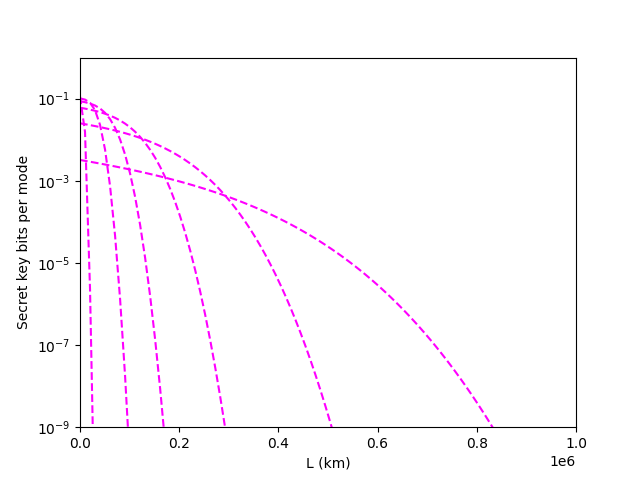
\includegraphics[width=0.6\linewidth]{figs/e_graph.png} 
    \caption{INSERT CAPTION HERE}
    \label{fig:e_caption}
\end{figure}
The probability of detecting a photon in one of the $m$ channels is given by $\epsilon_\text{trav}$ so the probability of at least one successful detection at the end is given by 
\begin{equation}
    P_\text{end} = 1 - (1-\eta^{1/(2n)}P_\text{chip}^{k+2}\eta_\text{GHZ}\eta_c).
\end{equation}
This gives us a formula for the rate per mode. For a given $m,k,b_0,b_1,$ the number of repeater stations $n$ can be optimized depending on the total distance of the repeater system. See figure \ref{fig:e_caption}. Notice that there is an envelope function. That is, the optimal $n$ changes depending on the length.
For a given $k$ we can optimize $m,b_0,b_1,n$ using grid search to obtain the maximum rate where condition \ref{eq:kmb-relation} is imposed. The optimal parameters for both the naive approach and the improved approach is summarized in table \ref{tab:table}.

\subsection{Naive Approach}
In the naive approach, there are a few changes.

\begin{table}
    \centering
    \begin{tabular}{|c|c|c|c|c|c|c|}
        \hline
        $k$ & $m_\text{naive}$ & $\vec{b}_\text{naive}$ & $R_\text{naive}$ & $m_\text{improved}$ & $\vec{b}_\text{improved}$ & $R_\text{naive}$ \\
        \hline
        7   & 5                & $[3, 2]$              & $1.91 \times 10^{-8}$ & 4                   & $[4, 2]$                 & $3.87 \times 10^{-6}$ \\
        8   & 8                & $[4, 2]$              & $6.13 \times 10^{-6}$ & 5                   & $[5, 3]$                 & $2.98 \times 10^{-3}$ \\
        9   & 11               & $[5, 3]$              & $5.77 \times 10^{-4}$ & 7                   & $[6, 4]$                 & $2.71 \times 10^{-2}$ \\
        10  & 13               & $[7, 4]$              & $7.42 \times 10^{-4}$ & 8                   & $[10, 5]$                & $4.93 \times 10^{-2}$ \\
        \hline
    \end{tabular}
    \caption{TABLE CAPTION HERE}
    \label{tab:table}
    \end{table}

\begin{itemize}
    \item Instead of having $2m$ parallel channels, the number of parallel channels change to 
    \begin{equation}
        N_\text{parallel} = 2m(b_0b_1+b_0+1).
    \end{equation}
    That is, all the qubits part of the attached trees become outer qubits and form channels.
    \item Because the mentioned qubits become outer qubits, they are transmitted through quantum channels instead, so all instances of $\epsilon_\text{stat}$ can be replaced with $\epsilon_\text{trav}.$
    \item Bell state measurements are done with less efficiency, and the success probability is given by 
    \begin{equation}
        P_B = \frac{1}{2} \cdot \left(P^{k+2}_\text{chip}\eta_\text{GHZ}\eta_c\right)^2 \cdot \eta^{1/n}
    \end{equation}
    instead.
\end{itemize}
\subsection{Analysis}
The optimal parameters in table \ref{tab:table} mostly agree with the ones found by Pant et al., with a few minor differences, which will be discussed in this section.
% \bibliographystyle{unsrt}%Used BibTeX style is unsrt
% \bibliography{sample}
\end{document}
